\scanpage{118}
\mspage{117}
\mspage{4}
\deleted{Soit} $i$

\deleted{L'introduction des $\Lambda_r^i$}

Fixons nous un indice dans $\{0,1,\infty\}$, disons $1$ (en pensant au cas où la triangulation est barycentrique, donc
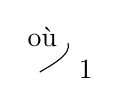
\begin{tikzpicture}[baseline=(one.base)]
\node[anchor=base west,inner sep=0pt] (one) at (.65,0) {$1$};
\node[anchor=base west,inner sep=0pt] at (0,.40) {\inserted{où}};
\draw[line width=.4pt] (.52,.45) .. controls (.57,.30) and (.29,.16) .. (.16,.08);
\end{tikzpicture}
joue un rôle particulier !). Nous pouvons éliminer les sommets $R_r^{ij}$ qui se trouvent sur des côtés de $r$ qui sont de type $1$, i.e. pour lesquels $i,j\ne1$, et l'arc $a_r^1$ qui les joint, en gardant les sommets
\[
(14)\qquad 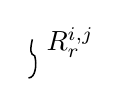
\begin{tikzpicture}[baseline=(rij.base)]
\node[inner sep=0pt] (rij) at (0,0) {$R_r^{i,j}$};
\draw[line width=.55pt] (-.48,.04) .. controls (-.51,-.09) and (-.51,-.15) .. (-.45,-.17)
  .. controls (-.42,-.28) and (-.44,-.45) .. (-.53,-.45);
\end{tikzpicture}\qquad
\left\{\begin{array}{l}
r\in\mathcal{R}\\
i\text{ ou }j\text{ est égal à }1\quad\text{i.e}\quad\{i,j\}\ne\{0,\infty\}
\end{array}\right.
\]
et les arcs
\[
(15)\qquad\left\{\begin{array}{ll}
\lambda_r^1&r\in\mathcal{R}\\
\Lambda_r^0,\Lambda_r^{\prime\infty}&r\in\mathcal{R},\quad\deleted{\unsure{i\in\{0,\infty\}}}\\
a_r^i&r\in\mathcal{R},\quad i\in\{0,\infty\}
\end{array}\right.
\]
\margin{$\Lambda_r^0\Lambda_{\tau_1r}^0=$}

avec comme relations les relations $(14)$ de
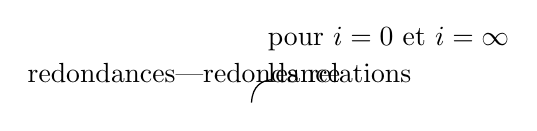
\begin{tikzpicture}[baseline=(red.base)]
\node[anchor=base west,inner sep=0pt] (red) at (0,0) {\unsure{redondances|redondance}};
\node[anchor=base west,inner sep=0pt] (oldwords) at (3.05,0) {\deleted{les relations}};
\node[anchor=base west,inner sep=0pt] at (3.05,.46) {\inserted{pour $i=0$ et $i=\infty$}};
\draw[line width=.45pt] (2.85,-.26) .. controls (2.86,-.04) and (2.99,.02) .. (3.10,.03);
\end{tikzpicture}
\deleted{du type $\unsure{\vcenter{\hbox{%
\begin{tikzpicture}[x=.55cm,y=.55cm]
\draw[line width=.45pt] (0.02,.65)..controls(0.03,.48)and(0.06,.30)..(0.015,.23)
 ..controls(-.02,.17)and(-.13,.20)..(-.12,.12)
 ..controls(-.10,.06)and(.07,.07)..(.08,-.04)
 ..controls(.10,-.12)and(.06,-.25)..(.13,-.26)--(.22,-.24);
\end{tikzpicture}}}}\Lambda_r^0=1$}

\figure{
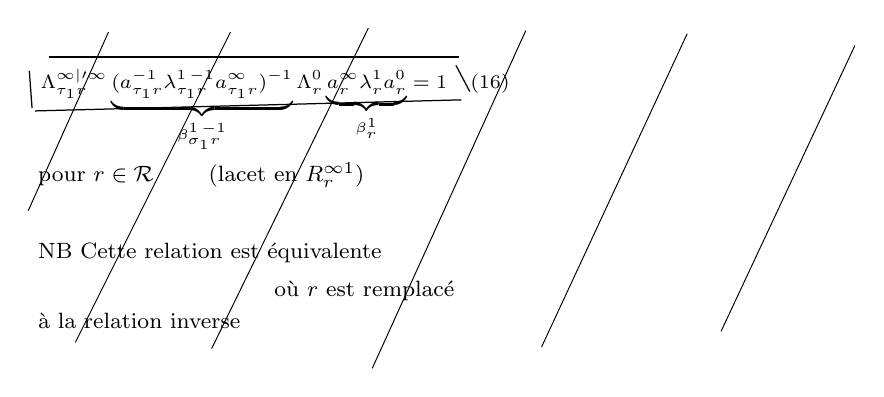
\begin{tikzpicture}[>=stealth]
\node[anchor=base west,inner sep=1pt,font=\scriptsize] (oldformula) at (0,0)
 {$\displaystyle \Lambda_{\unsure{\tau_1r}}^{\unsure{\infty|\prime\infty}}\underbrace{(a_{\tau_1r}^{-1}\lambda_{\tau_1r}^{1\,-1}a_{\tau_1r}^{\infty})^{-1}}_{\beta_{\sigma_1r}^{1\,-1}}\Lambda_r^0\underbrace{a_r^\infty\lambda_r^1a_r^0}_{\beta_r^1}=1$};
\node[anchor=base west,inner sep=0pt,font=\scriptsize] at ([xshift=7pt]oldformula.base east) {$(16)$};
\draw[line width=.45pt] ([xshift=4pt,yshift=3pt]oldformula.north west)
 -- ([xshift=3pt,yshift=3pt]oldformula.north east);
\draw[line width=.45pt] ([xshift=-3pt,yshift=-2pt]oldformula.north west)
 -- ([xshift=-2pt,yshift=-7pt]oldformula.base west);
\draw[line width=.45pt] ([xshift=-1pt,yshift=-8pt]oldformula.base west)
 -- ([xshift=4pt,yshift=-4pt]oldformula.base east);
\draw[line width=.45pt] ([xshift=2pt,yshift=0pt]oldformula.north east)
 -- ([xshift=7pt,yshift=-1pt]oldformula.base east);
\node[anchor=base west,inner sep=0pt,font=\footnotesize] at (0,-1.18)
 {pour $r\in\mathcal R$ \qquad (lacet en $R_r^{\infty1}$)};
\node[anchor=base west,inner sep=0pt,font=\footnotesize] at (0,-2.15)
 {\uline{NB} Cette relation est équivalente};
\node[anchor=base west,inner sep=0pt,font=\footnotesize] at (0,-3.05)
 {à la relation \deleted{\unsure{inverse}}};
\node[anchor=base west,inner sep=0pt,font=\footnotesize] at (3.00,-2.64)
 {\inserted{où $r$ est remplacé}};
% The six long cancellation strokes cross the formula and the prose together.
\draw[line width=.35pt] (.90,.72)--(-.12,-1.55);
\draw[line width=.35pt] (2.45,.72)--(.48,-3.22);
\draw[line width=.35pt] (4.20,.77)--(2.21,-3.30);
\draw[line width=.35pt] (6.20,.74)--(4.25,-3.55);
\draw[line width=.35pt] (8.25,.70)--(6.40,-3.28);
\draw[line width=.35pt] (10.38,.55)--(8.68,-3.08);
\end{tikzpicture}
}

\margin{pavage par des carrés ? (dont les sommets qui ne sont pas de type $1$, sont ``arrondis'', de façon à faire des hexagones évitant les trous}
\figure{
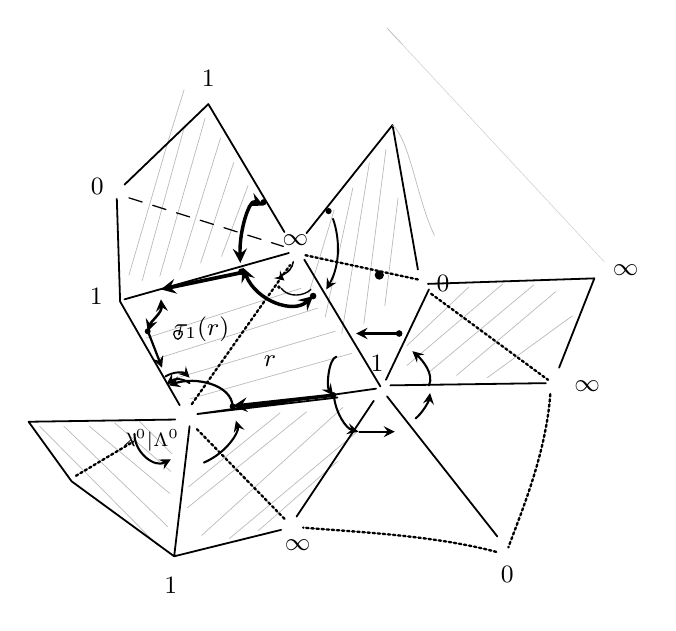
\begin{tikzpicture}[x=.014cm,y=-.014cm,>=stealth,line cap=round,line join=round]
\draw[gray!35,line width=.22pt] (595,1462)--(792,1674);
\draw[gray!50,line width=.22pt] (595,1462)--(609,1477);
% Light construction hatching: six local regions, with independently drawn strokes.
\draw[gray!55,line width=.25pt]
 (361,1686)--(397,1563)--(411,1518) (373,1691)--(412,1549) (389,1687)--(430,1544)
 (407,1681)--(444,1562) (426,1675)--(456,1584) (445,1669)--(469,1605);
\draw[gray!55,line width=.25pt]
 (524,1703)--(547,1627) (539,1724)--(564,1607) (554,1739)--(579,1584)
 (574,1730)--(594,1572) (593,1714)--(605,1616)
 (613,1750)--(669,1697) (613,1768)--(700,1694) (632,1775)--(728,1695)
 (658,1777)--(748,1701) (686,1779)--(763,1723)
 (377,1743)--(517,1698) (389,1761)--(532,1716) (402,1780)--(548,1737)
 (417,1798)--(563,1757)
 (414,1897)--(522,1810) (415,1878)--(498,1811) (427,1922)--(555,1806)
 (452,1925)--(568,1828) (478,1918)--(550,1855)
 (280,1823)--(387,1931) (302,1823)--(396,1914) (325,1823)--(398,1884)
 (348,1820)--(399,1864) (370,1818)--(400,1848);
% Solid edges stop separately around the punctured 0 and infinity corners.
\draw[line width=.65pt]
 (357,1604)--(433,1531)--(502,1647)
 (350,1617)--(353,1710)--(407,1804)
 (357,1708)--(506,1666)
 (520,1672)--(589,1787)
 (423,1812)--(585,1789)
 (416,1823)--(402,1941)
 (423,1812)--(550,1797)
 (522,1648)--(600,1550)--(623,1681)
 (632,1694)--(783,1689)--(751,1770)
 (633,1699)--(594,1781)
 (598,1786)--(739,1784)
 (595,1796)--(695,1923)
 (583,1800)--(513,1905)
 (499,1917)--(402,1941)--(309,1873)--(270,1819)--(403,1817);
\draw[gray!55,line width=.25pt] (600,1550)..controls(616,1564)and(622,1617)..(638,1650);
% The upper-left cross-edge uses long dashes, not dots.
\draw[dash pattern=on 5pt off 4pt,line width=.45pt] (361,1616)--(501,1660);
% The other cross-edges and outer continuation are dotted, with heavy round marks.
\draw[densely dotted,line width=.85pt]
 (521,1668)--(623,1690) (635,1703)--(741,1781)
 (743,1794)..controls(739,1850)and(715,1905)..(705,1933)
 (694,1937)..controls(638,1922)and(568,1919)..(519,1915)
 (502,1907)--(421,1824) (418,1803)--(507,1677)
 (313,1868)--(365,1837);
% Marked endpoints and thick directional paths at the top/left infinity corner.
\fill (483,1620) circle[radius=2.8];
\fill (542,1628) circle[radius=2.8];
\fill (588,1686) circle[radius=4.2];
\fill (463,1683) circle[radius=3.0];
\fill (528,1705) circle[radius=3.0];
\draw[line width=1.35pt,<-] (390,1699)--(462,1684);
\draw[line width=1.25pt,<->] (483,1623)..controls(470,1617)and(461,1646)..(462,1675);
\draw[line width=1.25pt,<->] (464,1679)..controls(477,1710)and(510,1721)..(528,1705);
\draw[line width=.7pt,->] (546,1635)..controls(552,1652)and(553,1676)..(540,1699);
\draw[line width=.55pt,->] (510,1674)..controls(508,1686)and(496,1686)..(502,1691);
\fill (497,1697) circle[radius=1.8];
\draw[line width=.5pt] (499,1698)..controls(506,1707)and(520,1705)..(526,1699);
% Two heads on the short left vertical arc; downward continuation below it.
\fill (378,1737) circle[radius=2.7];
\draw[line width=.9pt,<->] (390,1708)..controls(391,1720)and(381,1728)..(378,1737);
\draw[line width=.8pt,->] (379,1739)--(391,1770);
% Paired small arcs and the larger return around the lower central 0.
\draw[line width=.7pt,->] (394,1778)..controls(402,1773)and(411,1774)..(416,1779);
\draw[line width=.7pt,->] (416,1784)..controls(409,1779)and(402,1780)..(395,1785);
\draw[line width=.8pt,->] (455,1805)..controls(454,1785)and(421,1778)..(397,1786);
\fill (455,1805) circle[radius=2.7];
\fill (546,1795) circle[radius=3.0];
\draw[line width=1.3pt,<-] (455,1805)--(546,1795);
\draw[line width=.75pt,->] (549,1760)..controls(542,1762)and(540,1787)..(546,1795);
\draw[line width=.75pt,->] (429,1856)..controls(450,1847)and(461,1828)..(458,1818);
\draw[line width=.75pt,->] (366,1830)..controls(366,1847)and(384,1861)..(399,1853);
% Paths around the central 1 and beside its right edge.
\fill (606,1739) circle[radius=3.0];
\draw[line width=.8pt,<-] (567,1739)--(605,1739);
\draw[line width=.75pt,->] (633,1786)..controls(638,1776)and(627,1763)..(618,1755);
\draw[line width=.75pt,->] (621,1816)..controls(628,1810)and(633,1800)..(634,1793);
\draw[line width=.75pt,->] (547,1797)..controls(549,1812)and(558,1825)..(569,1828);
\draw[line width=.75pt,->] (570,1828)--(602,1828);
% Central labels. The small extra loop is preserved without calling it a deletion.
\node[font=\small] at (489,1764) {$r$};
\node[font=\small] at (427,1735) {$\tau_1(r)$};
\draw[line width=.45pt] (408,1737)..controls(402,1735)and(400,1738)..(403,1743)
 ..controls(406,1747)and(411,1740)..(409,1737);
\node[font=\scriptsize] at (381,1836) {$\unsure{\lambda^0|\Lambda^0}$};
% Every written vertex label, including both right-side infinity signs.
\node[font=\small,above] at (433,1524) {$1$};
\node[font=\small,left] at (347,1606) {$0$};
\node[font=\small,left] at (346,1705) {$1$};
\node[font=\small] at (512,1654) {$\infty$};
\node[font=\small,right] at (631,1694) {$0$};
\node[font=\small,right] at (791,1682) {$\infty$};
\node[font=\small,right] at (756,1787) {$\infty$};
\node[font=\small] at (586,1766) {$1$};
\node[font=\small,below] at (704,1941) {$0$};
\node[font=\small,below] at (514,1917) {$\infty$};
\node[font=\small,below] at (399,1951) {$1$};
\end{tikzpicture}
}

\[
(16)\qquad
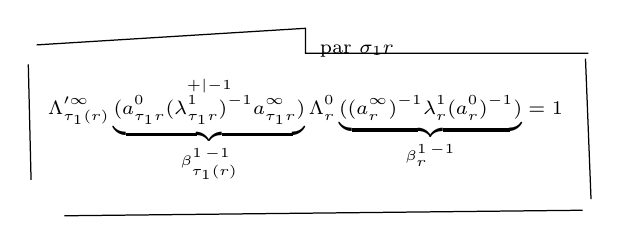
\begin{tikzpicture}[baseline=(live.base)]
\node[inner xsep=5pt,inner ysep=8pt,font=\scriptsize] (live)
 {$\displaystyle \Lambda_{\tau_1(r)}^{\prime\infty}\underbrace{(a_{\tau_1r}^{0}(\lambda_{\tau_1r}^1)^{-1}a_{\tau_1r}^{\infty})}_{\beta_{\tau_1(r)}^{1\,\deleted{\unsure{-1}}}}^{\unsure{+|-1}}\Lambda_r^0\underbrace{((a_r^\infty)^{-1}\lambda_r^1(a_r^0)^{-1})}_{\beta_r^{1\,-1}}=1$};
% Last words of the cancelled NB cross the new upper border at its notch.
\node[anchor=base west,inner sep=0pt,font=\scriptsize] at ([xshift=5pt]live.north)
 {par $\sigma_1r$};
\draw[line width=.45pt] ([xshift=1pt,yshift=3pt]live.north west)
 -- ([yshift=9pt]live.north) -- (live.north)
 -- ([xshift=4pt]live.north east);
\draw[line width=.45pt] ([xshift=3pt,yshift=-2pt]live.north east)
 -- ([xshift=5pt,yshift=2pt]live.south east);
\draw[line width=.45pt] ([xshift=2pt,yshift=-2pt]live.south east)
 -- ([xshift=11pt,yshift=-4pt]live.south west);
\draw[line width=.45pt] ([xshift=-2pt,yshift=-4pt]live.north west)
 -- ([xshift=-1pt,yshift=9pt]live.south west);
\end{tikzpicture}
\]
\margin{relation stable par passage de $r$ à $\tau_1(r)$, donc il suffit de la poser pour $r\in\mathcal{R}^+$ (si $X$ orientable)}
\figure{
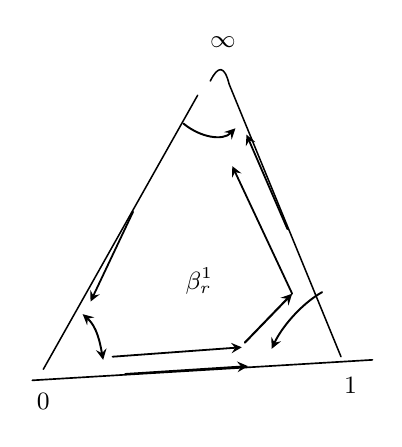
\begin{tikzpicture}[x=.020cm,y=-.020cm,>=stealth,line cap=round,line join=round]
% The side ends remain separate at the 0 and infinity corners.
\draw[line width=.55pt] (129,2127)--(31,2301);
\draw[line width=.55pt] (137,2118)..controls(142,2108)and(146,2108)..(149,2120)
 --(220,2293);
\draw[line width=.6pt] (24,2308)--(240,2295);
% Directions on the three outer sides.
\draw[line width=.65pt,->] (88,2201)--(61,2258);
\draw[line width=.7pt,->] (83,2304)--(161,2299);
\draw[line width=.65pt,->] (186,2212)--(160,2152);
% Interior path: a head at the bend as well as the upper endpoint.
\draw[line width=.65pt,->] (75,2293)--(157,2287);
\draw[line width=.75pt,->] (159,2284)--(189,2253);
\draw[line width=.65pt,->] (189,2253)--(151,2172);
% Three corner arcs, with both heads on the lower-left one.
\draw[line width=.7pt,->] (120,2145)..controls(131,2154)and(145,2156)..(153,2148);
\draw[line width=.7pt,<->] (56,2266)..controls(65,2274)and(67,2284)..(69,2295);
\draw[line width=.7pt,->] (208,2252)..controls(194,2260)and(182,2275)..(176,2288);
\node[font=\small] at (130,2245) {$\beta_r^1$};
\node[font=\small,above] at (145,2103) {$\infty$};
\node[font=\small,below] at (31,2310) {$0$};
\node[font=\small,below] at (226,2300) {$1$};
\end{tikzpicture}
}
